%\documentclass{sig-alternate-10pt}
\documentclass[11pt,twocolumn, oneside]{article} % use "amsart" instead of "article" for AMSLaTeX format
\usepackage{geometry}                		% See geometry.pdf to learn the layout options. There are lots.
\geometry{letterpaper}                   		% ... or a4paper or a5paper or ... 
\usepackage{longtable}
\usepackage{amsmath}
\usepackage{amssymb}
\usepackage{indentfirst}
\usepackage{graphicx}
\usepackage{hyperref}
\setlength{\oddsidemargin}{0in}
\setlength{\evensidemargin}{0in}
\setlength{\textheight}{9in}
\setlength{\textwidth}{6.5in}
\setlength{\topmargin}{-0.5in}
%\geometry{landscape}                		% Activate for for rotated page geometry
%\usepackage[parfill]{parskip}    		% Activate to begin paragraphs with an empty line rather than an indent
\usepackage{graphicx}				% Use pdf, png, jpg, or eps� with pdflatex; use eps in DVI mode
								% TeX will automatically convert eps --> pdf in pdflatex		
\usepackage{amssymb}

\title{\bf Project Report\\[2ex] 
 \rm\normalsize CSE223b --- Alex C. Snoeren --- Spring 2013}
\author{Ali Asghari, Amell Alghamdi}
\date{\today}							% Activate to display a given date or no date

\begin{document}
\maketitle

%%%%%%%%%%%%%%%%%%%%%%%%%%%%%%%%%%%%%%%%%%%%%%%%%%%
{\bf Abstract} - This paper presents a multicast system that guarantees a strong consistency among a small group of nodes, providing fault tolerance, while maintaining weaker consistency between the groups, which allows for greater performance. The system consists of key-value store that is built with a multicast protocol in conjunction with Gas Friends application, which is a simple interface that is used to show the functionality of the system. The papers proves by  experiments, that the system shows a significant enhancement in performance compared with the standard multicast protocol.

%%%%%%%%%%%%%%%%%%%%%%%%%%%%%%%%%%%%%%%%%%%%%%%%%%%%%%%%
\section{Introduction} 
Knowing the goal of the system is a key aspect to build an efficient system that meets the requirement of the system. This paper presents a multicast system that is built for Gas Friends (GF) application. GF�s main goal is to provide a fast and consistent updated for gas prices in each city in U.S .  That means, when a user open the application and choose San Diego city, if the user is in San Diego then he belongs to the set of primary users of San Diego page. The set of primary users will have a strong consistency view of the list of prices. On the other hand, users in different geographical locations such as New York are considered to be secondary users for San Diego prices� page, which means they will not �directly� benefit from San Diego page and, most probably, will not visit that page, then the need to have a strong consistent view could be compromised. Our system utilized this fact to enhance the performance by minimizing the round trip time, which is an important factor in transformation delay in other systems. 

%%%%%%%%%%%%%%%%%%%%%%%%%%%%%%%%%%%%%%%%%%%%%%%%%%%

\section{Motivation}
The system is developed taking in consideration the user as the center of the focus. In application like GF, the goal, mainly, is to serve the first tier users and this makes the application deals with different groups of users that are constructed according to the physical presents which ends up to have the same user to be a primary in one group and a secondary in another. The set up for those group was the real motivation to create such a system that broadcast the message to all users but to wait for the acknowledgment from the primary users only.    

%%%%%%%%%%%%%%%%%%%%%%%%%%%%%%%%%%%%%%%%%%%%%%%%

\section{Environment Set-up}

MiniNet  \cite{minimet} is the network simulation environment that we used to run the system, and it simulate a typical real-world network where netwrok failures can occur and may result in one or  more nodes being partitioned. On the other hand, we assume that a levers the seas a ware of  the subset for each Clique. In addition, we assume that the hard disc contents will never be lost. The language we used to implement the system is C++. The system interface (GF)is built with PHP.  The client-server that we implemented  are  implemented with thrift-0.9.0 and compiled with GCC 4.4.

%%%%%%%%%%%%%%%%%%%%%%%%%%%%%%%%%%%%%%%%%%%%%%%%%%%%%%%%
\section{Description of Our Multicast Protocol}
In general, the system consists of sets of Cliques; each set has a Master Node and a group of server nods. We believe that using a primary to commit data is more attractive than the standard two phase commit protocol since it alleviates the need to gather a majority quorum of servers \cite{bayou}. As a result, and by knowing the application's specifications, the system was built to adopt a week consistency outside the Clique and a strong one inside it. The client  sends a request to the Master Node, and the Master Node  multicasts  the request to all nods inside and outside its Clique, but the Master Node will wait for acknowledgment from the nods inside its Clique only.

\subsection{The Master Node}
The system will consist of number nodes (all trusted) each is independently accessible to outside clients. When a client accesses a node, that node is known as the Master Node for that client. At any given time there will be at most as many Master Nodes as clients in system, but may be fewer as multiple clients may share the same Master Node.  

\subsection{The Clique Nodes}
The nodes of the system will be organized into cliques of size n. A Master Node within a clique will multicast client requests to all nodes in the system, however will only require a response from member of it�s clique. If a clique member fails to reply in a designated time t, the Master Node will re-multicast the message and increase the timeout t by a random value before retrying. In the event a maximum number of retries are executed, the Master Node will select another node from the system to join it�s clique and continue if that node responds. In the event that n clique-mates cannot be found, the Master Node, for our purposes, will fail the client�s request. Note that this failure does not imply the message has not been committed by any nodes, simply that the Master Node cannot guarantee the fault tolerance agreement with the client. The master node will not advance its clock in the event of a failure.   

\subsection{The Non-Clique Nodes}
Nodes outside the clique may or may not receive messages, receive duplicate messages or receive messages out-of-order from Master Node. These will be handled silently by the non-clique members. Any messages received can be immediately committed. 

\subsection{The Heartbeat}
enforcing a global order on tentative as well as committed  messages ensure that isolated servers will come to agreement on resolution of any conflict  that they encounter \cite{bayou}.To ensure an individual node has not become completely isolated from the system, it will occasionally send a heartbeat request to a random node in the system along with it�s current vector clock. In the event the other nodes vector clock matches, an okay message is sent. In the event the two clocks don�t match the node with newest clock will send the last message it received which will cause the other node to initiate the algorithm described Fault Tolerance section.  

%%%%%%%%%%%%%%%%%%%%%%%%%%%%%%%%%%%%%%%%%%%%%%%%

\section{Fault Tolerance}
Since the system simulate the real-world network, fault tolerance is addressed. In the event a non-clique member hears a message from a Master Node which a timestamp significantly newer than the last known timestamp (i.e much high clock value), the node will assume it�s is missing data. To retrieve this data it will begin with it�s own clique-mates. In the event none of it�s clique -mates have the data, it will contact fixed number of nodes at random asking if any of them have the missing data. Lastly if all else fails, it will contact a node within the Master Node�s Clique (this set of nodes includes the Master Node) which is guaranteed to have the missing data since the Master Node will not send a new message until all of it�s clique-mates are up to speed. If a request makes it way all the way to the Master Node�s clique, it will be multicast to all nodes since if things got this far, it is assumed a number of other nodes are missing the data as well.

The major addition is to avoid to avoid the delay and communication overhead when loosing data. Applying this technique limit the scope of solicitations and repairs, in the hope of repairing problems where they occur \cite{twoScal}. One thing to note about this, is that by contacting other nodes asking for missing data, you are also spreading knowledge that data has gone missing. Any node receiving a message for which it cannot supply the missing data (since it is missing it as well) will begin with the same algorithm after a random delay to allow for the event that the original node will have to contact the Master Node�s clique and thus result in the re-multicasting of the message anyway.


%%%%%%%%%%%%%%%%%%%%%%%%%%%%%%%%%%%%%%%%%%%%%%%%

\section{Experiments}
The system has been tested using MiniNet  simulation environment. Two scenarios were tested. First, if the system send a multicast  message to all nodes and wait for acknowledgment from all nodes, Second, if the system send a multicast  message to a clique (subset group of nodes) and wait for acknowledgment from the nodes in the clique only. In the second scenario, the size of the clique is selected to be 5 ,10 and 15 nodes.


The result shows that by using cliques  we were able to reduce the time needed by factor of x in the case of 15 nodes, factor of y in case of  10 and by factor of z in case we used 5 nodes per clique. The result is demonstrated in Table \ref{tab:result}



		
    
   
   

\begin{table}\centering
  \begin{tabular}{| p{1.5cm} | c |c |c | c| }
   \hline
     Size of Clique	&  0	      &5 	                &10 	        &15 \\ \hline
     Sync Clique		& N/A			& 2 ns			& 2 ns			& 1.73 ns 		\\ \hline 
     Sync Sys		& N/A			& 4 ns			& 4 ns			& 3.33 ns  	\\ \hline 
     Latency		& N/A			& 4 ns			& 4 ns			& 3.33 ns  		\\ \hline 
     Standard Deviation & N/A			& 4 ns			& 4 ns			& 3.33 ns  \\ \hline 
  \end{tabular}
  \caption{Experiments' Result }
  \label{tab:result}
\end{table}



The following part should be removed at the end.
\begin{enumerate}
  \item Typical operation
   	\begin{itemize}
  		\item Time synchronize clique for various clique sizes
			\begin{itemize}
 				 \item Track number non-clique nodes which don�t receive the message
			\end{itemize}	  
 		 \item Time to synchronize total system ({\bf if time permits})
  		\item Typical latency
	\end{itemize}
  \item Partitioned system
          \begin{itemize}	  
 		 \item Number messages needed to repair after partition fixed
	\end{itemize}
  \item Induced latency
        \begin{itemize}	  
 		 \item How one slow in-clique node affects total client operation time
		 \item How one slow node outside the clique affects total client operation time
	\end{itemize}
\end{enumerate}
%%%%%%%%%%%%%%%%%%%%%%%%%%%%%%%%%%%%%%%%%%%%%%%%%

\section{Conclusion }
In our work environment where we insists on having a strong consistency among set of serveer nodes and a weaker consistency between the sets, the paper provided a customized multicast protocol that showed a great enhancement on the performance when it compared to the standard multicast protocol. 

\section{Future Work}
\subsection{The Synchronization Protocol}
Synchronization Protocol which will essentially enforce that all nodes, or a subset of nodes, synchronize all of their data before accepting any new client requests. 

\subsection{Choosing a Node }
Assuming a good number of nods that are connected to the same switch will get the same message from the multicast will give us the ability to choose different node in case of not getting a respond from a node in the Clique.

%%%%%%%% 
\begin{figure}
\centering
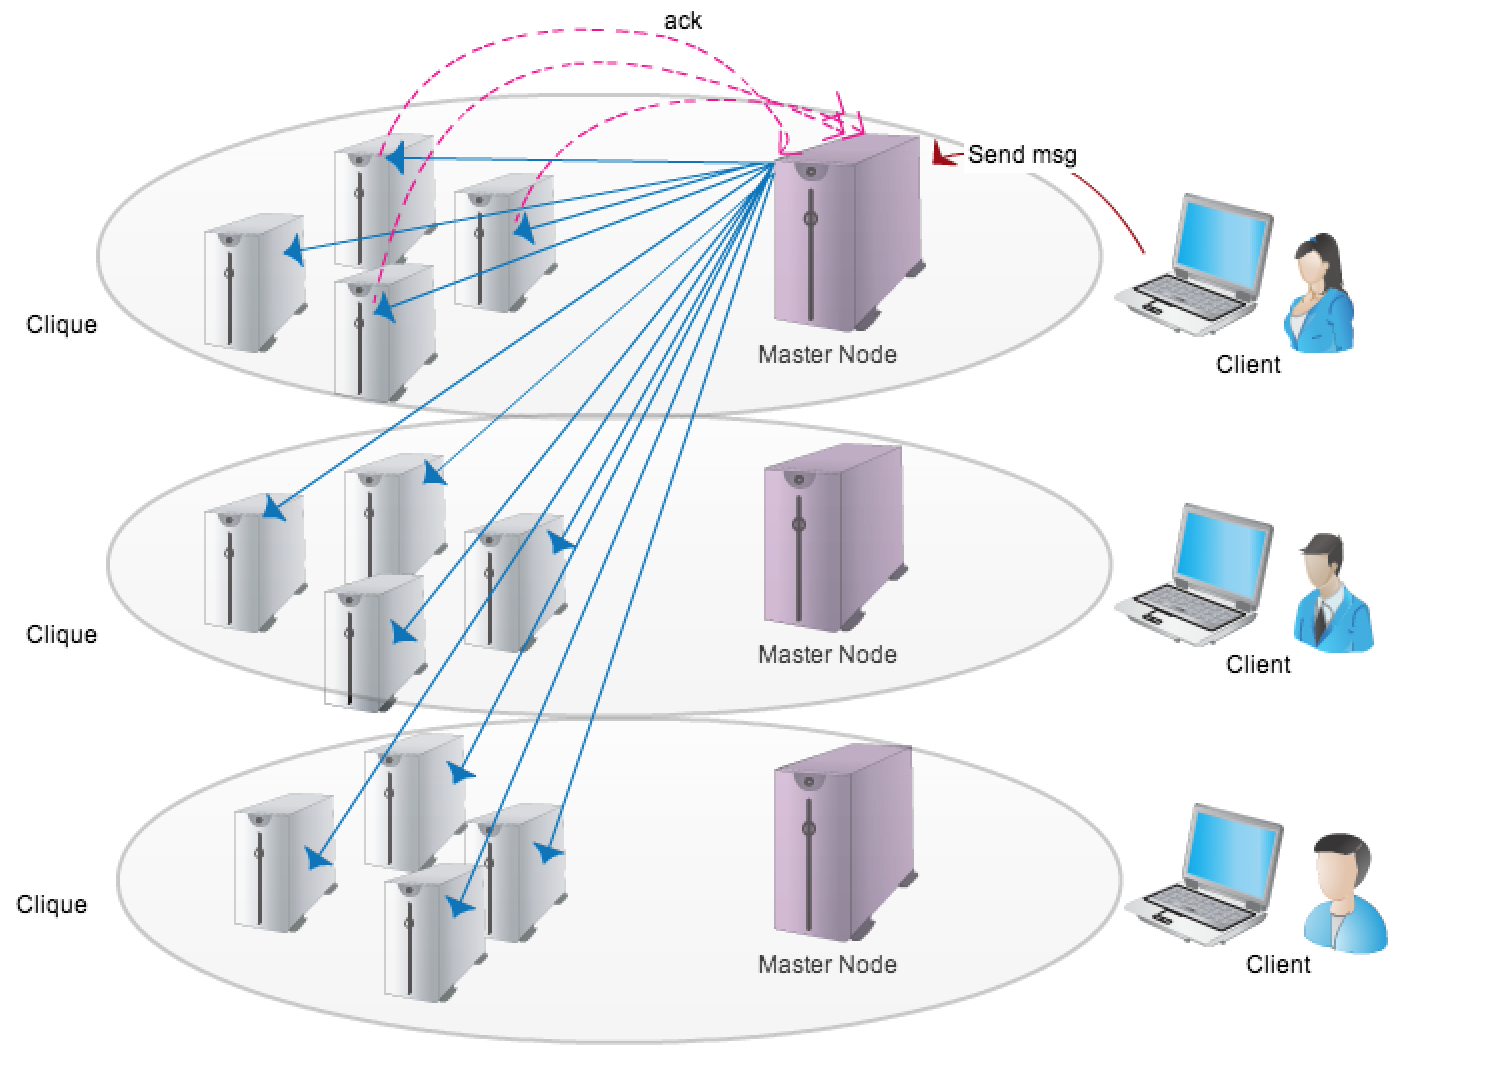
\includegraphics[scale=.4]{sys.png}
\label{fig:1-2}
\caption{Our System }
\end{figure}


%%%%%% list resources %%%%%%%%%%%%%
\begin{thebibliography}{4}
 	
 	\bibitem{bayou}
 		{\emph{Managing Update Conflicts in Bayou, a Weakly Connected Replicated Storage System} In Proceedings of the 15th ACM Symposium on Operating Systems Principles ({SOSP}-15), Copper Mountain Resort, Colorado (1995) by Douglas B. Terry, Marvin M. Theimer, Karin Petersen, et al.}	
	\bibitem{twoScal}
		{\emph{Scalability of Two Reliable Multicast Protocols}.Cornell University Ithaca, NY, USA(1999) by Oznur Ozkasap	, Zhen Xiao, and Kenneth P. Birman}	
		\bibitem{ns2}
 		\url{http://www.isi.edu/nsnam/ns/}
  	\bibitem{minimet}
 		\url{http://mininet.org}

\end{thebibliography}





\end{document}


